\hypertarget{Score_8cpp}{
\section{Score.cpp File Reference}
\label{Score_8cpp}\index{Score.cpp@{Score.cpp}}
}
{\tt \#include \char`\"{}Score.h\char`\"{}}\par
{\tt \#include \char`\"{}Types.h\char`\"{}}\par
{\tt \#include $<$vector$>$}\par
{\tt \#include $<$pthread.h$>$}\par


Include dependency graph for Score.cpp:\begin{figure}[H]
\begin{center}
\leavevmode
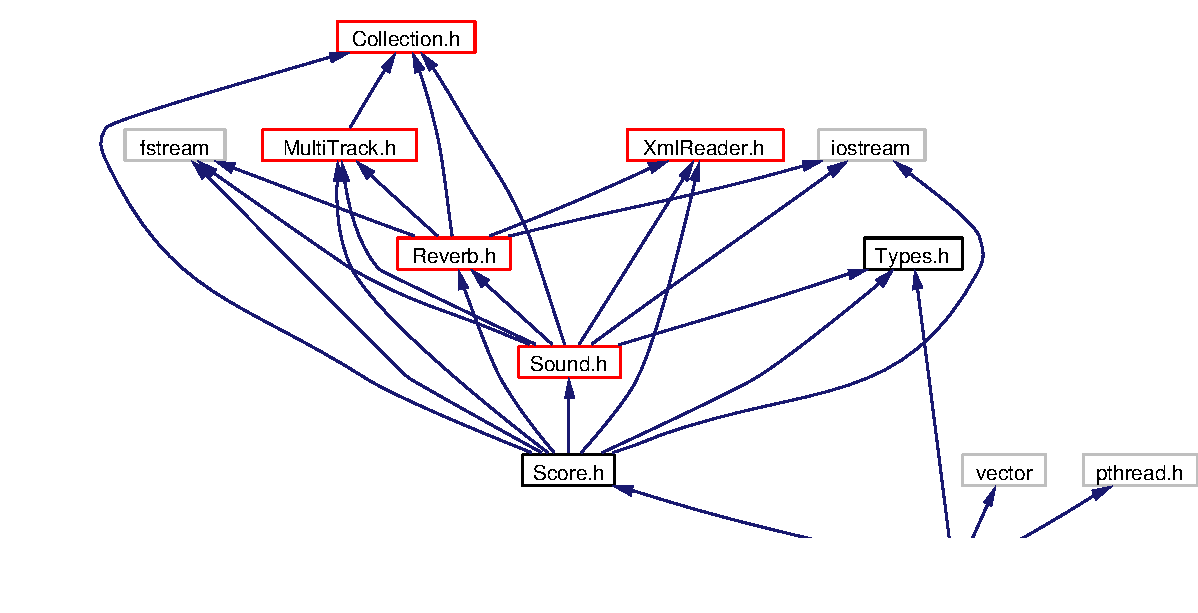
\includegraphics[width=305pt]{Score_8cpp__incl}
\end{center}
\end{figure}
\subsection*{Functions}
\begin{CompactItemize}
\item 
void $\ast$ \hyperlink{Score_8cpp_a0}{multithreaded\_\-render\_\-worker} (void $\ast$vtle)
\end{CompactItemize}


\subsection{Function Documentation}
\hypertarget{Score_8cpp_a0}{
\index{Score.cpp@{Score.cpp}!multithreaded_render_worker@{multithreaded\_\-render\_\-worker}}
\index{multithreaded_render_worker@{multithreaded\_\-render\_\-worker}!Score.cpp@{Score.cpp}}
\subsubsection[multithreaded\_\-render\_\-worker]{\setlength{\rightskip}{0pt plus 5cm}void$\ast$ multithreaded\_\-render\_\-worker (void $\ast$ {\em vtle})}}
\label{Score_8cpp_a0}




Definition at line 39 of file Score.cpp.

References threadlist\_\-entry::done, threadlist\_\-entry::finish\-Condition, threadlist\_\-entry::list\-Mutex, threadlist\_\-entry::num\-Channels, Sound::render(), threadlist\_\-entry::result\-Track, threadlist\_\-entry::sampling\-Rate, and threadlist\_\-entry::snd.

Referenced by Score::render().